\section{Lógica de Presentación: Los ViewModels}

La aplicación móvil se complementa y es orquestada por los ViewModels, que residen en el paquete `com.example.prueba3.Views`. Estos componentes son fundamentales en una arquitectura moderna de Android, ya que actúan como un puente robusto entre la interfaz de usuario (las pantallas de Jetpack Compose) y la lógica de negocio o las fuentes de datos. Su principal ventaja es que están diseñados para sobrevivir a los cambios de configuración del dispositivo (como rotaciones de pantalla), manteniendo el estado de la UI y los datos sin interrupciones.

Los ViewModels extienden la clase `androidx.lifecycle.ViewModel` y hacen un uso extensivo de las capacidades de concurrencia y gestión de estados de Kotlin Coroutines y Kotlin Flow para operaciones asíncronas y reactividad de datos.

\subsection{Tecnologías y Componentes Clave en ViewModels}

Para la gestión eficiente del estado de la interfaz de usuario y la ejecución de operaciones asíncronas, los ViewModels utilizan las siguientes tecnologías y componentes:

\begin{itemize}
	\item \textbf{`androidx.lifecycle.ViewModel`}: Es la clase base principal de la que heredan todos los ViewModels de la aplicación. Proporciona un ámbito de ciclo de vida (`viewModelScope`) que permite ejecutar operaciones asíncronas que se cancelan automáticamente cuando el ViewModel es destruido, evitando fugas de memoria.
	
	\item \textbf{`androidx.lifecycle.viewModelScope`}: Es un `CoroutineScope` predefinido que pertenece al ViewModel. Esto significa que cualquier coroutine lanzada dentro de `viewModelScope` se ejecutará en un hilo en segundo plano y se cancelará automáticamente si el ViewModel se destruye. Esto simplifica enormemente la gestión de operaciones de larga duración, como llamadas a la red o consultas a la base de datos.
	
	\item \textbf{`kotlinx.coroutines` (Coroutines):}
	Los ViewModels emplean Coroutines para manejar la asincronía de manera estructurada y concisa. Permiten escribir código asíncrono que parece síncrono, mejorando la legibilidad y la depuración. Las coroutines son esenciales para:
	\begin{itemize}
		\item `kotlinx.coroutines.launch`: Para iniciar una nueva coroutine en un `CoroutineScope` específico, como `viewModelScope`.
		\item `kotlinx.coroutines.Dispatchers`: Para especificar el hilo en el que se ejecutará una coroutine (e.g., `Dispatchers.IO` para operaciones de red o base de datos, `Dispatchers.Main` para actualizaciones de interfaz de usuario).
		\item `kotlinx.coroutines.withContext`: Para cambiar el contexto de ejecución de una coroutine a un `Dispatcher` diferente de manera segura, útil para alternar entre hilos de secundarios y el hilo principal.
	\end{itemize}
	
	\item \textbf{`kotlinx.coroutines.flow` (StateFlow y MutableStateFlow):}
	Los ViewModels gestionan el estado de la interfaz de usuario y exponen los datos de manera reactiva utilizando Kotlin Flow, específicamente:
	\begin{itemize}
		\item `kotlinx.coroutines.flow.MutableStateFlow<T>`: Es un tipo de `Flow` que puede emitir actualizaciones de estado mutables. Los ViewModels lo utilizan internamente para mantener el estado actual de la UI (ej., datos a mostrar, estado de carga, mensajes de error).
		\item `kotlinx.coroutines.flow.StateFlow<T>`: Es una versión de solo lectura de `MutableStateFlow`. Los ViewModels exponen sus `MutableStateFlow` internos como `StateFlow` a las Composables de la UI (`.asStateFlow()`). Esto garantiza que la interfaz de usuario solo pueda observar los cambios de estado, sin poder modificarlos directamente, promoviendo la inmutabilidad y una gestión de estado más segura.
	\end{itemize}
	
	\item \textbf{Manejo de Respuestas de API y Errores:}
	Para la interacción con las APIs y el procesamiento de respuestas, los ViewModels utilizan:
	\begin{itemize}
		\item `retrofit2.HttpException`: Esta excepción se utiliza para capturar y manejar errores específicos que ocurren durante las llamadas HTTP realizadas por Retrofit (por ejemplo, errores de servidor como 404, 500, etc.). Permite a los ViewModels reaccionar a problemas de red o de API de forma controlada.
		\item `org.json.JSONObject`: Se emplea para el análisis y la manipulación de datos en formato JSON, especialmente útil para extraer información de cuerpos de respuesta complejos o para construir cuerpos de solicitud.
	\end{itemize}
\end{itemize}

En resumen, los ViewModels son el corazón de la lógica de presentación, utilizando un conjunto robusto de herramientas de Jetpack y Kotlin Coroutines/Flow para gestionar el estado de la UI de forma eficiente, reactiva y segura, facilitando la comunicación con las capas de datos y la lógica de negocio del sistema.

\begin{figure}[htbp!]
	\begin{center}
		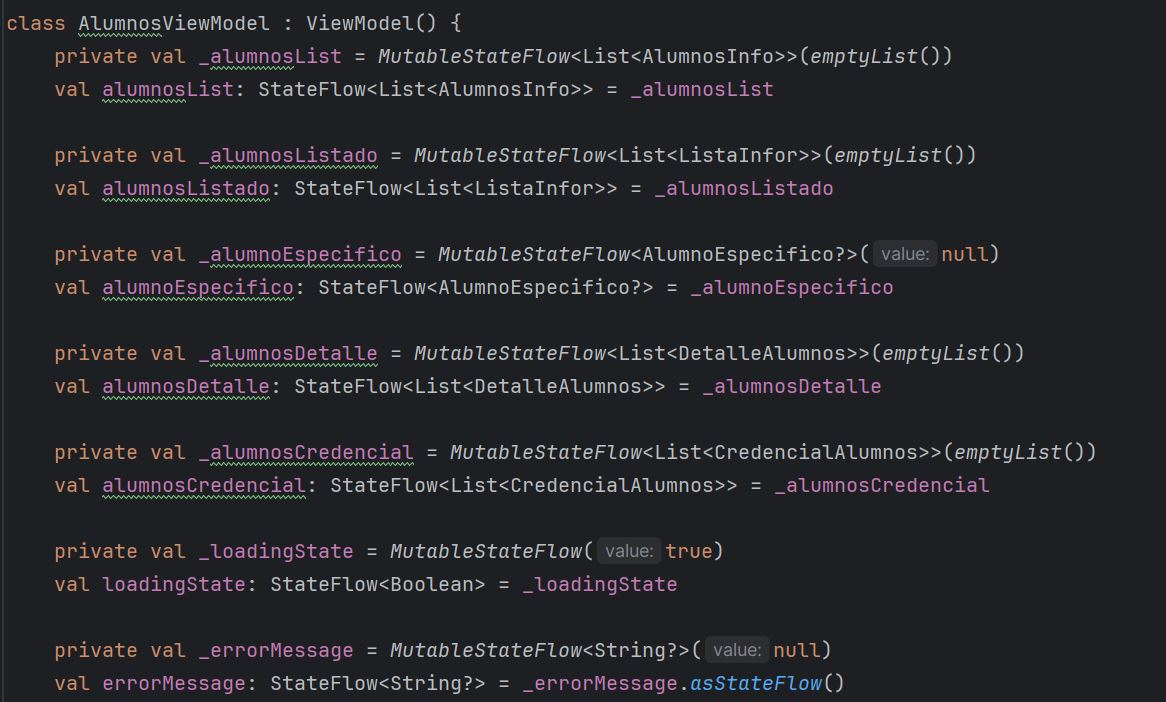
\includegraphics[width=0.9\textwidth]{ImagenesDetalles/Viewmodel1}
		\caption{Ejemplo de ViewModel AlumnosViewModel.kt donde se muestra la creación de un ViewModel y el uso de MutableStateFlow y StateFlow.}
		\label{fig:DetallesMovilViewmodel1}
	\end{center}
\end{figure}

\begin{figure}[htbp!]
	\begin{center}
		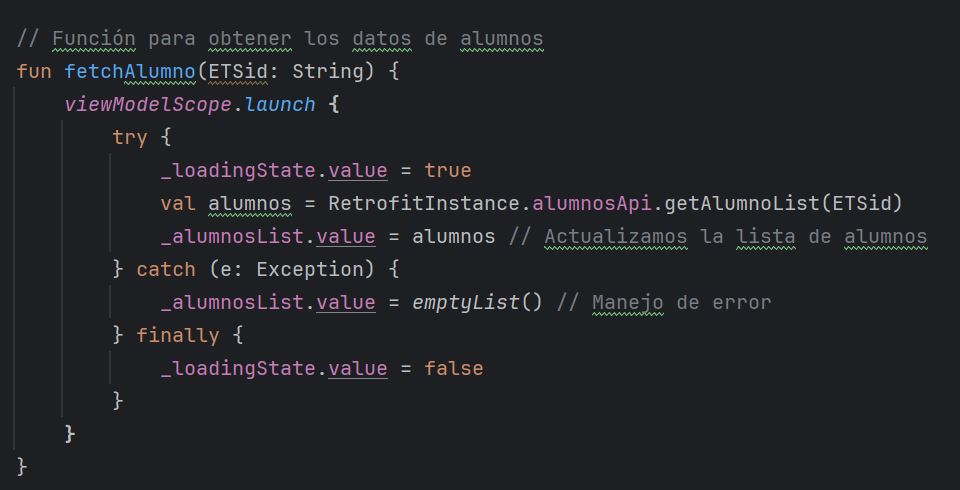
\includegraphics[width=0.9\textwidth]{ImagenesDetalles/Viewmodel2}
		\caption{Ejemplo de ViewModel AlumnosViewModel.kt donde se muestra el uso de viewModelScope y RetrofitInstance.}
		\label{fig:DetallesMovilViewmodel2}
	\end{center}
\end{figure}